\section{Spark::Sp\-Tuple4$<$ Real $>$ Class Template Reference}
\label{classSpark_1_1SpTuple4}\index{Spark::SpTuple4@{Spark::SpTuple4}}
{\tt \#include $<$Sp\-Tuple.h$>$}

Inheritance diagram for Spark::Sp\-Tuple4$<$ Real $>$:\begin{figure}[H]
\begin{center}
\leavevmode
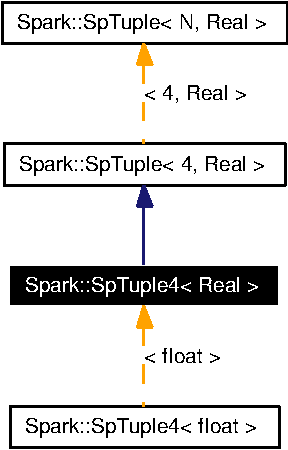
\includegraphics[width=86pt]{classSpark_1_1SpTuple4__inherit__graph}
\end{center}
\end{figure}
Collaboration diagram for Spark::Sp\-Tuple4$<$ Real $>$:\begin{figure}[H]
\begin{center}
\leavevmode
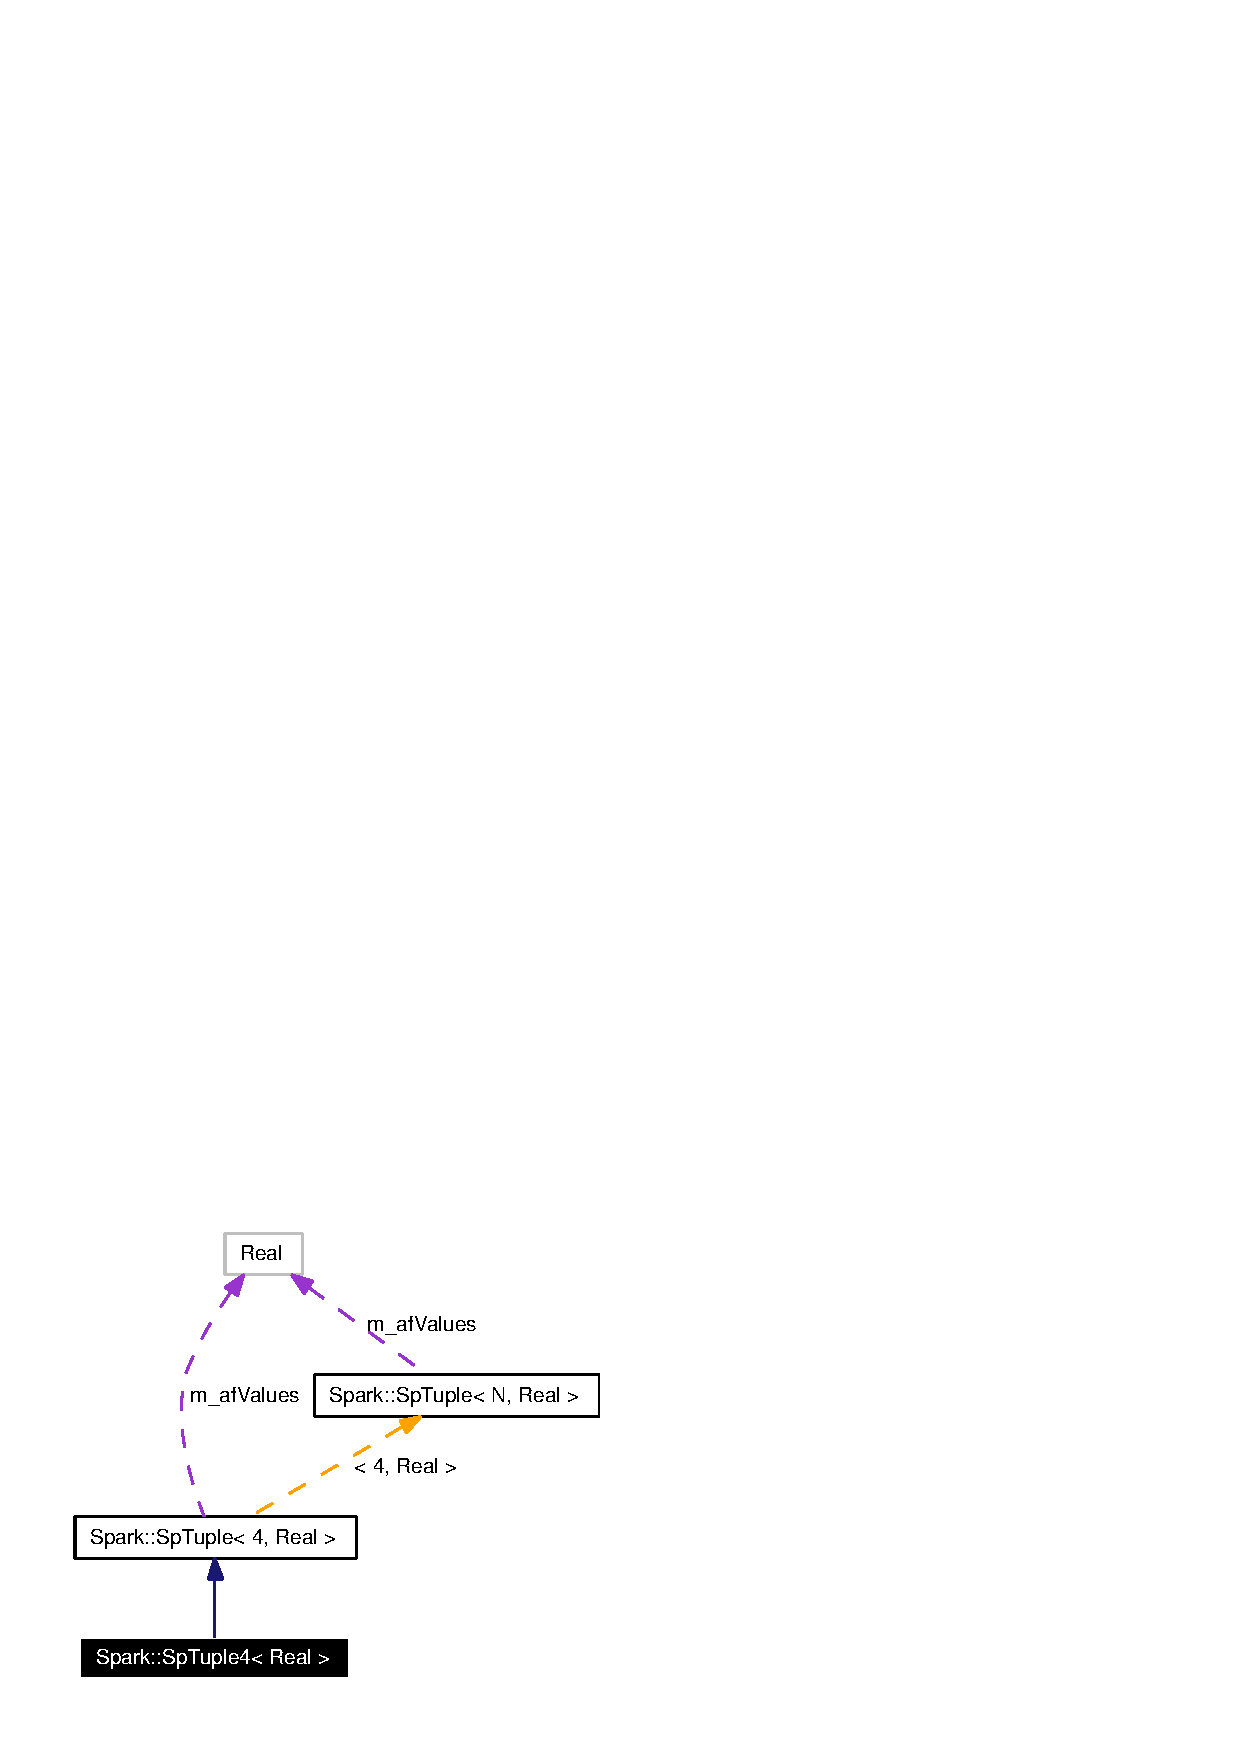
\includegraphics[width=144pt]{classSpark_1_1SpTuple4__coll__graph}
\end{center}
\end{figure}


\subsection{Detailed Description}
\subsubsection*{template$<$class Real$>$ class Spark::Sp\-Tuple4$<$ Real $>$}

4D tuple data class with support for vector mathematics 

Definition at line 188 of file Sp\-Tuple.h.\subsection*{Public Member Functions}
\begin{CompactItemize}
\item 
{\bf Sp\-Tuple4} (const {\bf Sp\-Tuple}$<$ 4, Real $>$ \&rk\-V)
\begin{CompactList}\small\item\em Construction. \item\end{CompactList}\item 
{\bf Sp\-Tuple4} (Real f\-X=0, Real f\-Y=0, Real f\-Z=0, Real f\-W=1)
\item 
Real {\bf x} () const
\begin{CompactList}\small\item\em Position Coordinate Access:. \item\end{CompactList}\item 
Real \& {\bf x} ()
\item 
Real {\bf y} () const
\item 
Real \& {\bf y} ()
\item 
Real {\bf z} () const
\item 
Real \& {\bf z} ()
\item 
Real {\bf w} () const
\item 
Real \& {\bf w} ()
\item 
Real {\bf r} () const
\begin{CompactList}\small\item\em Color Component Access:. \item\end{CompactList}\item 
Real \& {\bf r} ()
\item 
Real {\bf g} () const
\item 
Real \& {\bf g} ()
\item 
Real {\bf b} () const
\item 
Real \& {\bf b} ()
\item 
Real {\bf a} () const
\item 
Real \& {\bf a} ()
\item 
Real {\bf s} () const
\begin{CompactList}\small\item\em Texture Coordinate Access:. \item\end{CompactList}\item 
Real \& {\bf s} ()
\item 
Real {\bf t} () const
\item 
Real \& {\bf t} ()
\item 
Real {\bf p} () const
\item 
Real \& {\bf p} ()
\item 
Real {\bf q} () const
\item 
Real \& {\bf q} ()
\end{CompactItemize}


\subsection{Constructor \& Destructor Documentation}
\index{Spark::SpTuple4@{Spark::Sp\-Tuple4}!SpTuple4@{SpTuple4}}
\index{SpTuple4@{SpTuple4}!Spark::SpTuple4@{Spark::Sp\-Tuple4}}
\subsubsection{\setlength{\rightskip}{0pt plus 5cm}template$<$class Real$>$ {\bf Spark::Sp\-Tuple4}$<$ Real $>$::{\bf Sp\-Tuple4} (const {\bf Sp\-Tuple}$<$ 4, Real $>$ \& {\em rk\-V})\hspace{0.3cm}{\tt  [inline]}}\label{classSpark_1_1SpTuple4_a0}


Construction. 

Definition at line 194 of file Sp\-Tuple.h.\index{Spark::SpTuple4@{Spark::Sp\-Tuple4}!SpTuple4@{SpTuple4}}
\index{SpTuple4@{SpTuple4}!Spark::SpTuple4@{Spark::Sp\-Tuple4}}
\subsubsection{\setlength{\rightskip}{0pt plus 5cm}template$<$class Real$>$ {\bf Spark::Sp\-Tuple4}$<$ Real $>$::{\bf Sp\-Tuple4} (Real {\em f\-X} = {\tt 0}, Real {\em f\-Y} = {\tt 0}, Real {\em f\-Z} = {\tt 0}, Real {\em f\-W} = {\tt 1})\hspace{0.3cm}{\tt  [inline]}}\label{classSpark_1_1SpTuple4_a1}


Definition at line 197 of file Sp\-Tuple.h.

\subsection{Member Function Documentation}
\index{Spark::SpTuple4@{Spark::Sp\-Tuple4}!a@{a}}
\index{a@{a}!Spark::SpTuple4@{Spark::Sp\-Tuple4}}
\subsubsection{\setlength{\rightskip}{0pt plus 5cm}template$<$class Real$>$ Real\& {\bf Spark::Sp\-Tuple4}$<$ Real $>$::a ()\hspace{0.3cm}{\tt  [inline]}}\label{classSpark_1_1SpTuple4_a17}


Definition at line 222 of file Sp\-Tuple.h.\index{Spark::SpTuple4@{Spark::Sp\-Tuple4}!a@{a}}
\index{a@{a}!Spark::SpTuple4@{Spark::Sp\-Tuple4}}
\subsubsection{\setlength{\rightskip}{0pt plus 5cm}template$<$class Real$>$ Real {\bf Spark::Sp\-Tuple4}$<$ Real $>$::a () const\hspace{0.3cm}{\tt  [inline]}}\label{classSpark_1_1SpTuple4_a16}


Definition at line 221 of file Sp\-Tuple.h.

Referenced by Spark::Sp\-Window::draw\-String().\index{Spark::SpTuple4@{Spark::Sp\-Tuple4}!b@{b}}
\index{b@{b}!Spark::SpTuple4@{Spark::Sp\-Tuple4}}
\subsubsection{\setlength{\rightskip}{0pt plus 5cm}template$<$class Real$>$ Real\& {\bf Spark::Sp\-Tuple4}$<$ Real $>$::b ()\hspace{0.3cm}{\tt  [inline]}}\label{classSpark_1_1SpTuple4_a15}


Definition at line 220 of file Sp\-Tuple.h.\index{Spark::SpTuple4@{Spark::Sp\-Tuple4}!b@{b}}
\index{b@{b}!Spark::SpTuple4@{Spark::Sp\-Tuple4}}
\subsubsection{\setlength{\rightskip}{0pt plus 5cm}template$<$class Real$>$ Real {\bf Spark::Sp\-Tuple4}$<$ Real $>$::b () const\hspace{0.3cm}{\tt  [inline]}}\label{classSpark_1_1SpTuple4_a14}


Definition at line 219 of file Sp\-Tuple.h.

Referenced by Spark::Sp\-Window::draw\-String().\index{Spark::SpTuple4@{Spark::Sp\-Tuple4}!g@{g}}
\index{g@{g}!Spark::SpTuple4@{Spark::Sp\-Tuple4}}
\subsubsection{\setlength{\rightskip}{0pt plus 5cm}template$<$class Real$>$ Real\& {\bf Spark::Sp\-Tuple4}$<$ Real $>$::g ()\hspace{0.3cm}{\tt  [inline]}}\label{classSpark_1_1SpTuple4_a13}


Definition at line 218 of file Sp\-Tuple.h.\index{Spark::SpTuple4@{Spark::Sp\-Tuple4}!g@{g}}
\index{g@{g}!Spark::SpTuple4@{Spark::Sp\-Tuple4}}
\subsubsection{\setlength{\rightskip}{0pt plus 5cm}template$<$class Real$>$ Real {\bf Spark::Sp\-Tuple4}$<$ Real $>$::g () const\hspace{0.3cm}{\tt  [inline]}}\label{classSpark_1_1SpTuple4_a12}


Definition at line 217 of file Sp\-Tuple.h.

Referenced by Spark::Sp\-Window::draw\-String().\index{Spark::SpTuple4@{Spark::Sp\-Tuple4}!p@{p}}
\index{p@{p}!Spark::SpTuple4@{Spark::Sp\-Tuple4}}
\subsubsection{\setlength{\rightskip}{0pt plus 5cm}template$<$class Real$>$ Real\& {\bf Spark::Sp\-Tuple4}$<$ Real $>$::p ()\hspace{0.3cm}{\tt  [inline]}}\label{classSpark_1_1SpTuple4_a23}


Definition at line 232 of file Sp\-Tuple.h.\index{Spark::SpTuple4@{Spark::Sp\-Tuple4}!p@{p}}
\index{p@{p}!Spark::SpTuple4@{Spark::Sp\-Tuple4}}
\subsubsection{\setlength{\rightskip}{0pt plus 5cm}template$<$class Real$>$ Real {\bf Spark::Sp\-Tuple4}$<$ Real $>$::p () const\hspace{0.3cm}{\tt  [inline]}}\label{classSpark_1_1SpTuple4_a22}


Definition at line 231 of file Sp\-Tuple.h.\index{Spark::SpTuple4@{Spark::Sp\-Tuple4}!q@{q}}
\index{q@{q}!Spark::SpTuple4@{Spark::Sp\-Tuple4}}
\subsubsection{\setlength{\rightskip}{0pt plus 5cm}template$<$class Real$>$ Real\& {\bf Spark::Sp\-Tuple4}$<$ Real $>$::q ()\hspace{0.3cm}{\tt  [inline]}}\label{classSpark_1_1SpTuple4_a25}


Definition at line 234 of file Sp\-Tuple.h.\index{Spark::SpTuple4@{Spark::Sp\-Tuple4}!q@{q}}
\index{q@{q}!Spark::SpTuple4@{Spark::Sp\-Tuple4}}
\subsubsection{\setlength{\rightskip}{0pt plus 5cm}template$<$class Real$>$ Real {\bf Spark::Sp\-Tuple4}$<$ Real $>$::q () const\hspace{0.3cm}{\tt  [inline]}}\label{classSpark_1_1SpTuple4_a24}


Definition at line 233 of file Sp\-Tuple.h.\index{Spark::SpTuple4@{Spark::Sp\-Tuple4}!r@{r}}
\index{r@{r}!Spark::SpTuple4@{Spark::Sp\-Tuple4}}
\subsubsection{\setlength{\rightskip}{0pt plus 5cm}template$<$class Real$>$ Real\& {\bf Spark::Sp\-Tuple4}$<$ Real $>$::r ()\hspace{0.3cm}{\tt  [inline]}}\label{classSpark_1_1SpTuple4_a11}


Definition at line 216 of file Sp\-Tuple.h.\index{Spark::SpTuple4@{Spark::Sp\-Tuple4}!r@{r}}
\index{r@{r}!Spark::SpTuple4@{Spark::Sp\-Tuple4}}
\subsubsection{\setlength{\rightskip}{0pt plus 5cm}template$<$class Real$>$ Real {\bf Spark::Sp\-Tuple4}$<$ Real $>$::r () const\hspace{0.3cm}{\tt  [inline]}}\label{classSpark_1_1SpTuple4_a10}


Color Component Access:. 

Definition at line 215 of file Sp\-Tuple.h.

Referenced by Spark::Sp\-Window::draw\-String().\index{Spark::SpTuple4@{Spark::Sp\-Tuple4}!s@{s}}
\index{s@{s}!Spark::SpTuple4@{Spark::Sp\-Tuple4}}
\subsubsection{\setlength{\rightskip}{0pt plus 5cm}template$<$class Real$>$ Real\& {\bf Spark::Sp\-Tuple4}$<$ Real $>$::s ()\hspace{0.3cm}{\tt  [inline]}}\label{classSpark_1_1SpTuple4_a19}


Definition at line 228 of file Sp\-Tuple.h.\index{Spark::SpTuple4@{Spark::Sp\-Tuple4}!s@{s}}
\index{s@{s}!Spark::SpTuple4@{Spark::Sp\-Tuple4}}
\subsubsection{\setlength{\rightskip}{0pt plus 5cm}template$<$class Real$>$ Real {\bf Spark::Sp\-Tuple4}$<$ Real $>$::s () const\hspace{0.3cm}{\tt  [inline]}}\label{classSpark_1_1SpTuple4_a18}


Texture Coordinate Access:. 

Definition at line 227 of file Sp\-Tuple.h.\index{Spark::SpTuple4@{Spark::Sp\-Tuple4}!t@{t}}
\index{t@{t}!Spark::SpTuple4@{Spark::Sp\-Tuple4}}
\subsubsection{\setlength{\rightskip}{0pt plus 5cm}template$<$class Real$>$ Real\& {\bf Spark::Sp\-Tuple4}$<$ Real $>$::t ()\hspace{0.3cm}{\tt  [inline]}}\label{classSpark_1_1SpTuple4_a21}


Definition at line 230 of file Sp\-Tuple.h.\index{Spark::SpTuple4@{Spark::Sp\-Tuple4}!t@{t}}
\index{t@{t}!Spark::SpTuple4@{Spark::Sp\-Tuple4}}
\subsubsection{\setlength{\rightskip}{0pt plus 5cm}template$<$class Real$>$ Real {\bf Spark::Sp\-Tuple4}$<$ Real $>$::t () const\hspace{0.3cm}{\tt  [inline]}}\label{classSpark_1_1SpTuple4_a20}


Definition at line 229 of file Sp\-Tuple.h.\index{Spark::SpTuple4@{Spark::Sp\-Tuple4}!w@{w}}
\index{w@{w}!Spark::SpTuple4@{Spark::Sp\-Tuple4}}
\subsubsection{\setlength{\rightskip}{0pt plus 5cm}template$<$class Real$>$ Real\& {\bf Spark::Sp\-Tuple4}$<$ Real $>$::w ()\hspace{0.3cm}{\tt  [inline]}}\label{classSpark_1_1SpTuple4_a9}


Definition at line 210 of file Sp\-Tuple.h.\index{Spark::SpTuple4@{Spark::Sp\-Tuple4}!w@{w}}
\index{w@{w}!Spark::SpTuple4@{Spark::Sp\-Tuple4}}
\subsubsection{\setlength{\rightskip}{0pt plus 5cm}template$<$class Real$>$ Real {\bf Spark::Sp\-Tuple4}$<$ Real $>$::w () const\hspace{0.3cm}{\tt  [inline]}}\label{classSpark_1_1SpTuple4_a8}


Definition at line 209 of file Sp\-Tuple.h.

Referenced by Spark::Sp\-Tuple4$<$ float $>$::Sp\-Tuple4().\index{Spark::SpTuple4@{Spark::Sp\-Tuple4}!x@{x}}
\index{x@{x}!Spark::SpTuple4@{Spark::Sp\-Tuple4}}
\subsubsection{\setlength{\rightskip}{0pt plus 5cm}template$<$class Real$>$ Real\& {\bf Spark::Sp\-Tuple4}$<$ Real $>$::x ()\hspace{0.3cm}{\tt  [inline]}}\label{classSpark_1_1SpTuple4_a3}


Definition at line 204 of file Sp\-Tuple.h.\index{Spark::SpTuple4@{Spark::Sp\-Tuple4}!x@{x}}
\index{x@{x}!Spark::SpTuple4@{Spark::Sp\-Tuple4}}
\subsubsection{\setlength{\rightskip}{0pt plus 5cm}template$<$class Real$>$ Real {\bf Spark::Sp\-Tuple4}$<$ Real $>$::x () const\hspace{0.3cm}{\tt  [inline]}}\label{classSpark_1_1SpTuple4_a2}


Position Coordinate Access:. 

Definition at line 203 of file Sp\-Tuple.h.

Referenced by Spark::Sp\-Tuple4$<$ float $>$::Sp\-Tuple4().\index{Spark::SpTuple4@{Spark::Sp\-Tuple4}!y@{y}}
\index{y@{y}!Spark::SpTuple4@{Spark::Sp\-Tuple4}}
\subsubsection{\setlength{\rightskip}{0pt plus 5cm}template$<$class Real$>$ Real\& {\bf Spark::Sp\-Tuple4}$<$ Real $>$::y ()\hspace{0.3cm}{\tt  [inline]}}\label{classSpark_1_1SpTuple4_a5}


Definition at line 206 of file Sp\-Tuple.h.\index{Spark::SpTuple4@{Spark::Sp\-Tuple4}!y@{y}}
\index{y@{y}!Spark::SpTuple4@{Spark::Sp\-Tuple4}}
\subsubsection{\setlength{\rightskip}{0pt plus 5cm}template$<$class Real$>$ Real {\bf Spark::Sp\-Tuple4}$<$ Real $>$::y () const\hspace{0.3cm}{\tt  [inline]}}\label{classSpark_1_1SpTuple4_a4}


Definition at line 205 of file Sp\-Tuple.h.

Referenced by Spark::Sp\-Tuple4$<$ float $>$::Sp\-Tuple4().\index{Spark::SpTuple4@{Spark::Sp\-Tuple4}!z@{z}}
\index{z@{z}!Spark::SpTuple4@{Spark::Sp\-Tuple4}}
\subsubsection{\setlength{\rightskip}{0pt plus 5cm}template$<$class Real$>$ Real\& {\bf Spark::Sp\-Tuple4}$<$ Real $>$::z ()\hspace{0.3cm}{\tt  [inline]}}\label{classSpark_1_1SpTuple4_a7}


Definition at line 208 of file Sp\-Tuple.h.\index{Spark::SpTuple4@{Spark::Sp\-Tuple4}!z@{z}}
\index{z@{z}!Spark::SpTuple4@{Spark::Sp\-Tuple4}}
\subsubsection{\setlength{\rightskip}{0pt plus 5cm}template$<$class Real$>$ Real {\bf Spark::Sp\-Tuple4}$<$ Real $>$::z () const\hspace{0.3cm}{\tt  [inline]}}\label{classSpark_1_1SpTuple4_a6}


Definition at line 207 of file Sp\-Tuple.h.

Referenced by Spark::Sp\-Tuple4$<$ float $>$::Sp\-Tuple4().

The documentation for this class was generated from the following file:\begin{CompactItemize}
\item 
{\bf Sp\-Tuple.h}\end{CompactItemize}
